%!TEX root = ../template.tex
%%%%%%%%%%%%%%%%%%%%%%%%%%%%%%%%%%%%%%%%%%%%%%%%%%%%%%%%%%%%%%%%%%%
%% chapter1.tex
%% NOVA thesis document file
%%
%% Chapter with introduction
%%%%%%%%%%%%%%%%%%%%%%%%%%%%%%%%%%%%%%%%%%%%%%%%%%%%%%%%%%%%%%%%%%%

\typeout{NT FILE chapter1.tex}%

\chapter{X-ray Tracing}
\label{cha:xray_tracing}

\par Computed Tomography (CT) imaging is a critical diagnostic tool used by medical professionals to diagnose various illnesses and injuries. While the use of CT imaging is essential to provide immediate, life-saving results, ionizing radiation can damage cells and increase the risk of cancer. While the risk is small, it is cumulative, so physicians must track a patient's radiation exposure over time \cite{lauer2009elements}. Typically, exposure is measured using absorbed dose in the body and air kerma at the skin layer, which both have units of grays (joule/kg), making it directly related to the energy deposited by photons and their secondary particles. Often, these values are estimated based on the properties of the x-ray source and the specific procedure being performed. However, the most accurate estimation techniques use Monte Carlo (MC) methods to simulate the propagation of photons through a computational phantom \cite{essmedphys2012}. 
\par In the MC technique, the 3D space encompassing the phantom and the radiation source is represented as a computational domain. Within this domain, individual photon interactions are stochastically simulated, accounting for each interaction event as photons navigate the phantom. Such stochastic simulation offers unparalleled precision, capturing even the most subtle nuances of radiation behavior in biological media. Additionally, the MC method can simulate various medium types, densities, and configurations, making it incredibly versatile and adaptable to various imaging tests. Furthermore, advancements in computational power and algorithms have expedited MC simulation, rendering it more accessible and feasible for routine clinical applications \cite{fernandez_bosman_validation_2021}.
\par In this paper, the newly developed, open-source MC photon transport code system MIDSX is presented and validated. While many existing MC transport code systems perform reliably in dosimetry applications \cite{fernandez_bosman_validation_2021, geant4valid2004}, many of these systems are tailored for general particle transport. The developmental focus of MIDSX on x-ray transport reduces the complexity of implementation and allows users to easily design and run simulations specifically relating to x-ray transport in the medical imaging energy range. The subsequent sections will delve into the theory of MIDSX, compare results from MIDSX to accepted benchmarks from established simulation systems, and outline future work.

\section{Ray Tracing}
\par Ray tracing is a computer graphics technique that involves tracing the path of rays as they pass through a virtual scene. Due to its ability to create highly-realistic images, it has been used extensively in animations, video games, scientific computing, and by designers who need a physically accurate design of a product. While not the only rendering technique or the fastest in computer graphics, its ability to consistently produce physically realistic renders has made it an indispensable tool in many industries. By accurately simulating the behavior of light, ray tracing can capture intricate details of how light interacts with objects, resulting in realistic shadows, reflections, refractions, and global illumination effects. This level of visual fidelity allows for the creation of visually stunning and immersive experiences that were previously challenging to achieve. As hardware capabilities continue to advance and real-time ray tracing becomes more accessible, its applications are expanding, and its impact on various fields is growing, pushing the boundaries of what is possible in computer graphics and visual simulation. \cite{Peddie}

\subsection{The Brute Force Algorithm}

The rays in a scene are described mathematically as the parametric representation of a line. In three dimensions, the point at the end of the line $\va*{r}$ at parameter $t$ is given by the following equation:

\begin{equation}
\va*{r}(t) = \va*{r_0} + \vu*{d} t,
\label{eq:parametric_ray}
\end{equation}

\noindent where $\va*{r_0}$ points from the origin to the start of the line and $\vu*{d}$ is a unit vector parallel to the direction of the line. The described ray is shown in Figure \ref{fig:ray_diagram}.\\

\begin{figure}[H]
    \centering
	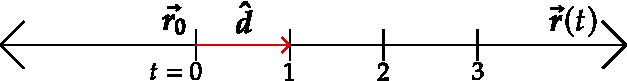
\includegraphics[width=\textwidth]{RayDiagram.pdf}
	\caption{A diagram of a parametric ray.}
	\label{fig:ray_diagram}
\end{figure}

\par Unlike in real life where light rays end at a camera, we instead trace light rays from the camera to locations in the scene. While one could trace light rays from a light source (forward ray tracing), many of these rays would end up missing the camera entirely, not affecting the image. More efficiently, the light rays are instead traced from the camera to the light source (backward ray tracing), drastically cutting back on the computational load while producing an identical image for most practical cases. \cite{Peddie} So, in the case of backward ray tracing, the method used in this research, rays are emitted from the camera; therefore, $\va*{r_0}$ represents the location of the camera in the scene.

\par To define the area of the scene visible from the point of view of the camera, one can create a rectangular area in which all rays pass through, called a viewport. Increasing the size of the viewport increases the amount of the scene that is visible in the final image, and vice versa. This viewport is broken up into a grid, the resolution of which determines the resolution of the final image. Rays are then sent through each point in this grid and out into the scene.

\par So far, we have a camera, light rays, and a way to define what parts of the scene are visible; all three of which are visualized in Figure \ref{fig:basic_ray_tracing_setup}. It is important to note that, by convention, the $z$-axis in the scene points opposite the viewport.

\begin{figure}[H]
  \centering
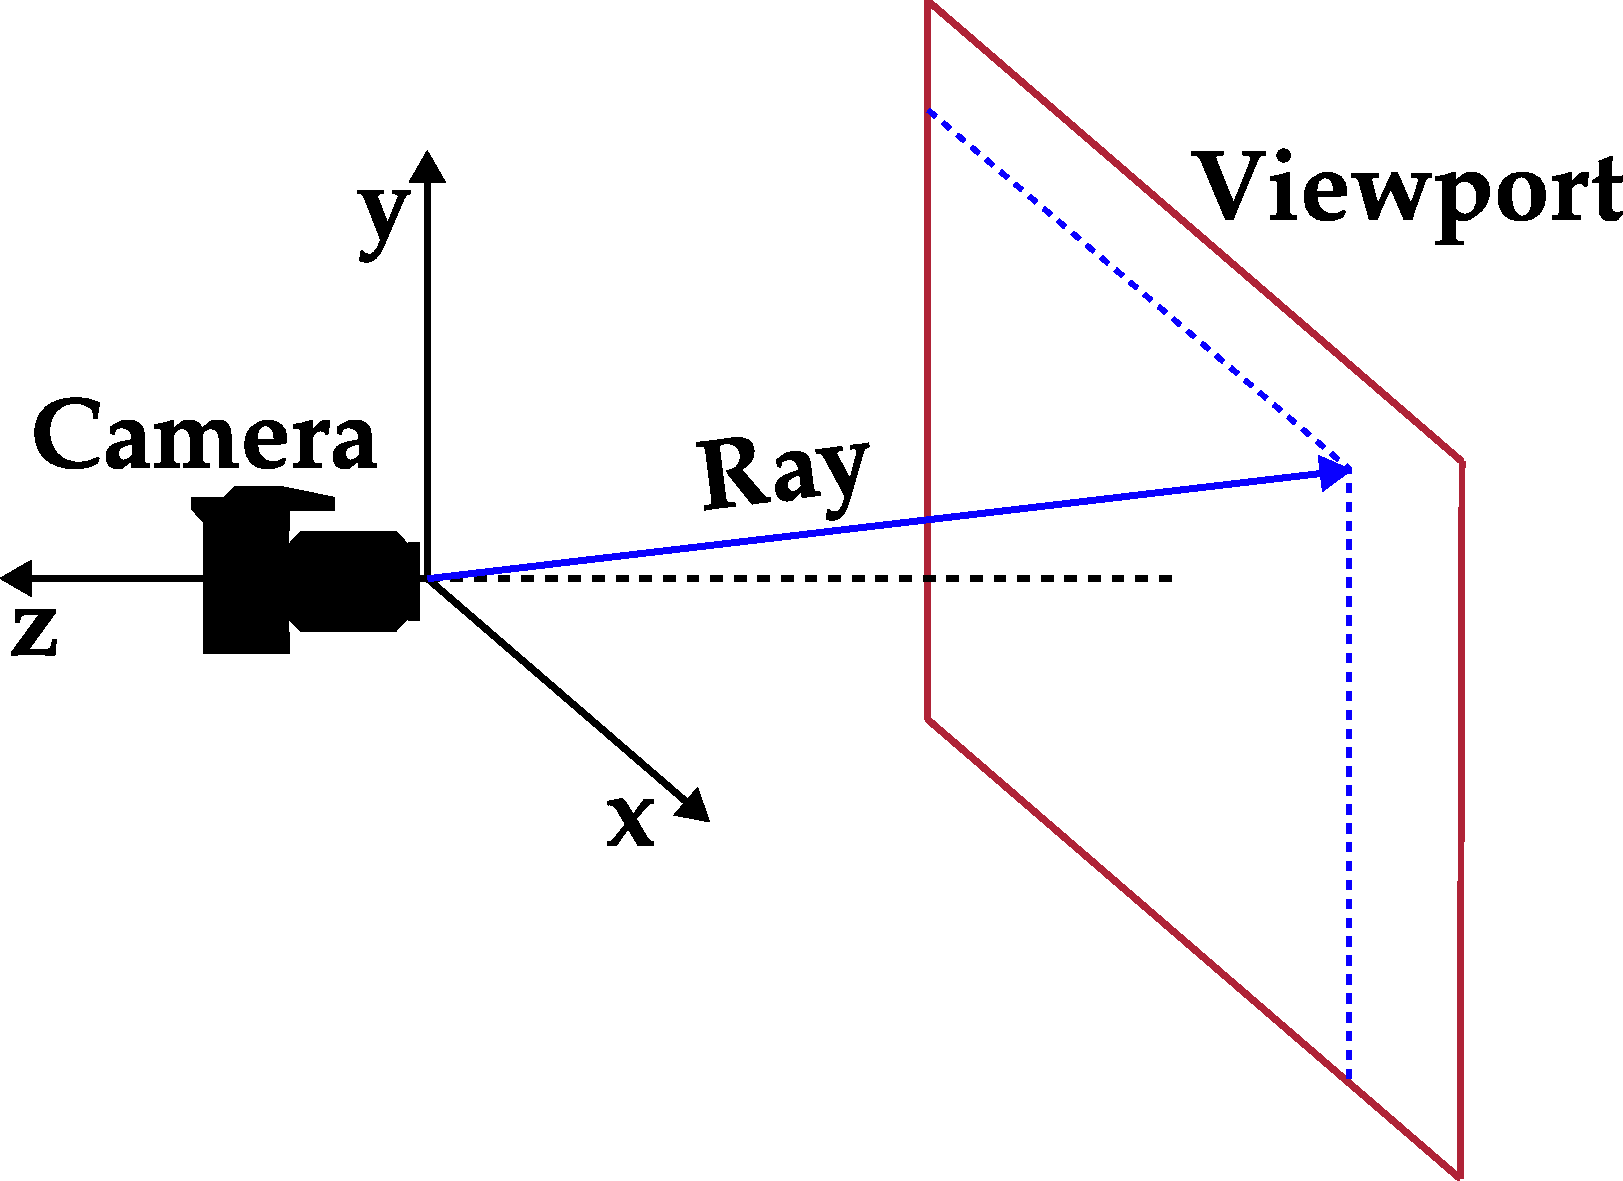
\includegraphics[width=\textwidth]{RayTracingSetup.pdf}
\caption{A basic ray-tracing setup with a camera, ray, and viewport.}
\label{fig:basic_ray_tracing_setup}
\end{figure}

\par To set the location of the viewport in the scene, we must first define three new vectors: $\val{HO}$, $\val{VE}$, and $\val{FL}$, which are vectors pointing from the left most to right most point (-$x$ to $x$ direction), the bottom most to top most point (-$y$ to $y$ direction), and from the center of the viewport to $\va*{r_0}$, respectively. A vector pointing from $\va*{r_0}$, to the bottom-left corner $\val{LHC}$ can be calculated using the following equation:

\begin{equation}
  \val{LHC} = \va*{r_0} - \frac{1}{2}\val{HO} - \frac{1}{2}\val{VE} - \val{FL},
  \label{eq:LHC}
\end{equation}

\noindent which was obtained visually from Figure \ref{fig:LHC_diagram}. \cite{Shirley}

\begin{figure}[H]
    \centering
	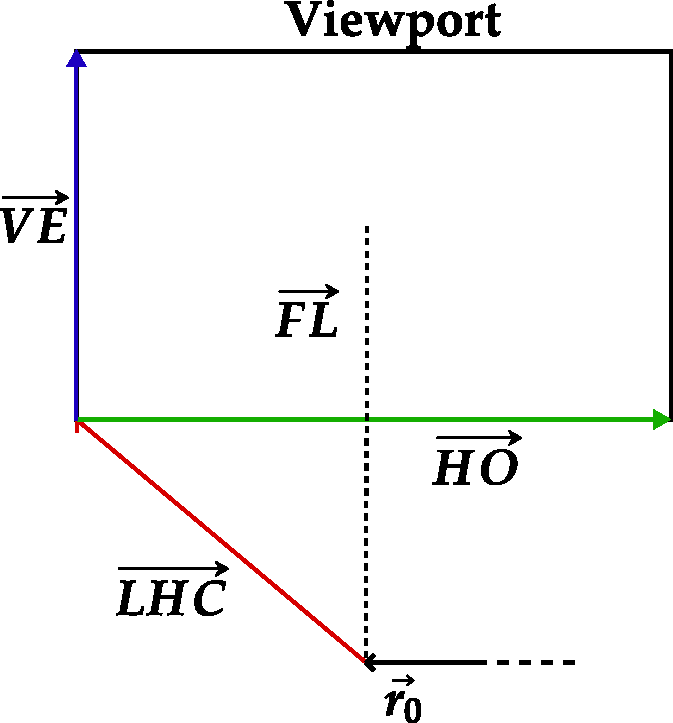
\includegraphics[width = 0.8\textwidth]{LHCDiagram.pdf}
	\caption{A diagram showing the geometric representations of $\protect\val{HO}$, $\protect\val{VE}$,
   $\protect\val{FL}$, and $\protect\val{LHC}$ with respect to the viewport.}
	\label{fig:LHC_diagram}
\end{figure}

\par With $\val{LHC}$ pointing to the left-hand-corner of the viewport in the scene, $\val{HO}$ and $\val{VE}$ can be scaled to define a ray pointing from the camera to any point on the viewport. In particular,  the viewport's horizontal and vertical coordinates, $u$ and $v$, are defined as such,

\begin{align}
u &= i/(\text{image width} - 1),\\
v &= j/(\text{image height} - 1),
\label{eq:viewport_coords}
\end{align}

\noindent where the image width and height are the resolution of the rendered image, $i$ is an integer ranging from [0, image width - 1], and $j$ is an integer ranging from [0, pixel height - 1]. Note that both $u$ and $v$ range from [0, 1].

\par Therefore, using these newly defined viewport coordinates, a ray taking the form of Equation \ref{eq:parametric_ray}, pointing from the camera to the pixel coordinates $(i, j)$ is given by the following equation:

\begin{equation}
  \va*{r}{\bm{i,j}}(t) = \va*{r_0} + t \left( \val{LHC} + u_i \val{HO}  + v_j \val{VE} - \val{A} \right),
  \label{eq:ray_to_viewport}
\end{equation}

\noindent which is represented geometrically in Figure \ref{fig:ray_to_viewport_diagram}. \cite{Shirley}

\begin{figure}[H]
  \centering
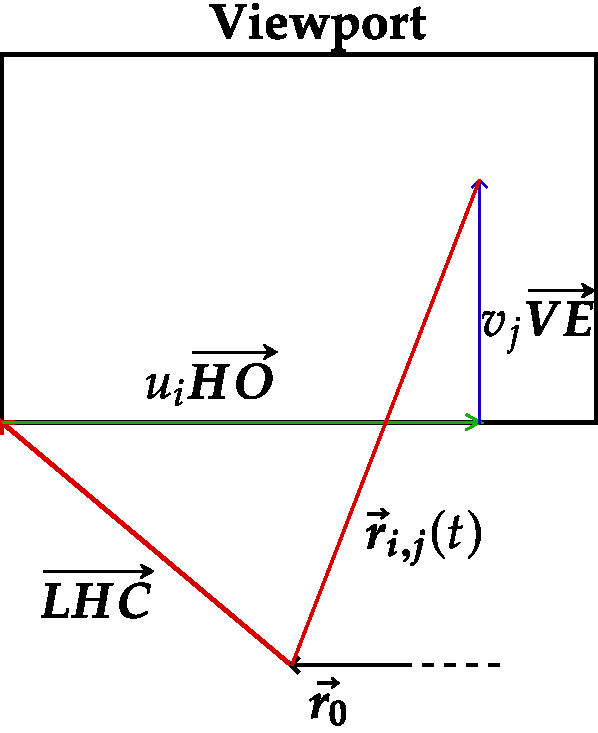
\includegraphics[width = 0.8\textwidth]{RayToViewportDiagram.pdf}
\caption{A diagram showing the geometric representation of Equation \ref{eq:ray_to_viewport}.}
\label{fig:ray_to_viewport_diagram}
\end{figure}

